\procTitle{Четырёхвершинники полуполевой проективной плоскости порядка~16}
\procAuthor{Степанюк~Г.\,А.}
\procEmail{glebstepanyk1998@gmail.com}
\procOrganization{СВГУ} \procCity{Магадан}

\makeProcTitle
\index{s@Степанюк~Г.\,А.}

\textbf{Введение}

Выявление строения конечных проективных плоскостей является актуальным направлением исследования. Так, например, в работе [1] развивается подход к построению и классификации полуполевых проективных плоскостей с использованием регулярного множества. В~статье [3] исследуются аффинные ельмслевовые плоскости, изучаются проективные плоскости, координатизируемые конечными почти-полями, квазиполями [2, 4].

Цель исследования~--- выявить особенности отношения инцидентности точек и прямых полуполевой проективной плоскости порядка 16. Рассматриваются множества пяти точек общего положения (никакие три не лежат на одной
прямой). Используя такие пять точек в качестве вершин, получаем пять четырёхвершинников. Известно, что полуполевая проективная плоскость порядка 16 допускает как обыкновенные четырёхвершинники, так и четырёхвершинники Фано. Подтверждается гипотеза, что для любого $k \in 0,1,2,3,4,5$ существуют конфигурации, в которых число обыкновенных четырёхвершинников и четырёхвершинников Фано равно $k$ и $5-k$ соответственно.

\textbf{Методы и результаты}

Проективной плоскостью называется инцидентностная структура $(P, L, I)$, если выполняются следующие аксиомы:

\begin{description}[noitemsep]\vspace{-6pt}
\item[А1.] Для любых двух различных точек существует единственная инцидентная им прямая;
\item[А2.] Для любых двух различных прямых существует единственная инцидентная им точка;
\item[А3.] Существуют хотя по крайней мере точки, любые три из которых не~инцидентны.
\end{description}\vspace{-8pt}

\begin{table}
\caption{Таблица Кэли полуполя $S^1_{16}=(S_{16},+,\circ)$}
\label{tab:zhelydeva}
\begin{changemargin}{-2cm}{0cm}
\begin{tabular}{p{0.7cm}|p{0.5cm}p{0.5cm}p{0.5cm}p{0.5cm}p{0.5cm}p{0.5cm}p{0.5cm}p{0.5cm}p{0.5cm}p{0.5cm}p{0.5cm}p{0.5cm}p{0.5cm}p{0.5cm}p{0.5cm}p{0.5cm}}
$\circ$     & (0;0) & (0;1) & (0;$\upalpha$) & (0;$\upbeta$) & (1;0) & (1;1) & (1;$\upalpha$) & (1;$\upbeta$) & ($\upalpha$;0) & ($\upalpha$;1) & ($\upalpha$;$\upalpha$) & ($\upalpha$;$\upbeta$) & ($\upbeta$;0) & ($\upbeta$;1) & ($\upbeta$;$\upalpha$) & ($\upbeta$;$\upbeta$) \\\hline


(0;0) & (0;0) & (0;0) & (0;0) & (0;0) & (0;0) & (0;0) & (0;0) & (0;0) & (0;0) & (0;0) & (0;0) & (0;0) & (0;0) & (0;0) & (0;0) & (0;0) \\
(0;1) & (0;0) & (1;1) & ($\upalpha$;$\upbeta$) & ($\upbeta$;$\upalpha$) & (0;1) & (1;0) & ($\upalpha$;$\upalpha$) & ($\upbeta$;$\upbeta$) & (0;$\upalpha$) & (1;$\upbeta$) & ($\upalpha$;1) & ($\upbeta$;0) & (0;$\upbeta$) & (1;$\upalpha$) & ($\upalpha$;0) & ($\upbeta$;1) \\
(0;$\upalpha$) & (0;0) & ($\upbeta$;$\upbeta$) & (1;$\upalpha$) & ($\upalpha$;1) & (0;$\upalpha$) & ($\upbeta$;1) & (1;0) & ($\upalpha$;$\upbeta$) & (0;$\upbeta$) & ($\upbeta$;0) & (1;1) & ($\upalpha$;$\upalpha$) & (0;1) & ($\upbeta$;$\upalpha$) & (1;$\upbeta$) & ($\upalpha$;0) \\
(0;$\upbeta$) & (0;0) & ($\upalpha$;$\upalpha$) & ($\upbeta$;1) & (1;$\upbeta$) & (0;$\upbeta$) & ($\upalpha$;1) & ($\upbeta$;$\upalpha$) & (1;0) & (0;1) & ($\upalpha$;$\upbeta$) & ($\upbeta$;0) & (1;$\upalpha$) & (0;$\upalpha$) & ($\upalpha$;0) & ($\upbeta$;$\upbeta$) & (1;1) \\
(1;0) & (0;0) & (0;1) & (0;$\upalpha$) & (0;$\upbeta$) & (1;0) & (1;1) & (1;$\upalpha$) & (1;$\upbeta$) & ($\upalpha$;0) & ($\upalpha$;1) & ($\upalpha$;$\upalpha$) & ($\upalpha$;$\upbeta$) & ($\upbeta$;0) & ($\upbeta$;1) & ($\upbeta$;$\upalpha$) & ($\upbeta$;$\upbeta$) \\
(1;1) & (0;0) & (1;0) & ($\upalpha$;1) & ($\upbeta$;1) & (1;1) & (0;1) & ($\upbeta$;0) & ($\upalpha$;0) & ($\upalpha$;$\upalpha$) & ($\upbeta$;$\upalpha$) & (0;$\upbeta$) & (1;$\upbeta$) & ($\upbeta$;$\upbeta$) & ($\upalpha$;$\upbeta$) & (1;$\upalpha$) & (0;$\upalpha$) \\
(1;$\upalpha$) & (0;0) & ($\upbeta$;$\upalpha$) & (1;0) & ($\upalpha$;$\upalpha$) & (1;$\upalpha$) & ($\upalpha$;0) & (0;$\upalpha$) & ($\upbeta$;0) & ($\upalpha$;$\upbeta$) & (1;1) & ($\upbeta$;$\upbeta$) & (0;1) & ($\upbeta$;1) & (0;$\upbeta$) & ($\upalpha$;1) & (1;$\upbeta$) \\
(1;$\upbeta$) & (0;0) & ($\upalpha$;$\upbeta$) & ($\upbeta$;$\upbeta$) & (1;0) & (1;$\upbeta$) & ($\upbeta$;0) & ($\upalpha$;0) & (0;$\upbeta$) & ($\upalpha$;1) & (0;$\upalpha$) & (1;$\upalpha$) & ($\upbeta$;1) & ($\upbeta$;$\upalpha$) & (1;1) & (0;1) & ($\upalpha$;$\upalpha$) \\
($\upalpha$;0) & (0;0) & (0;$\upbeta$) & (0;1) & (0;$\upalpha$) & ($\upalpha$;0) & ($\upalpha$;$\upbeta$) & ($\upalpha$;1) & ($\upalpha$;$\upalpha$) & ($\upbeta$;0) & ($\upbeta$;$\upbeta$) & ($\upbeta$;1) & ($\upbeta$;$\upalpha$) & (1;0) & (1;$\upbeta$) & (1;1) & (1;$\upalpha$) \\
($\upalpha$;1) & (0;0) & (1;0) & ($\upalpha$;$\upbeta$) & ($\upbeta$;0) & ($\upalpha$;1) & ($\upbeta$;$\upbeta$) & (0;$\upbeta$) & (1;$\upalpha$) & ($\upbeta$;$\upalpha$) & ($\upalpha$;0) & (1;1) & (0;$\upalpha$) & (1;$\upbeta$) & (0;1) & ($\upbeta$;1) & ($\upalpha$;$\upalpha$) \\
($\upalpha$;$\upalpha$) & (0;0) & ($\upbeta$;0) & (1;$\upbeta$) & ($\upalpha$;$\upbeta$) & ($\upalpha$;$\upalpha$) & (1;$\upalpha$) & ($\upbeta$;1) & (0;1) & ($\upbeta$;$\upbeta$) & (0;$\upalpha$) & ($\upalpha$;0) & (1;0) & (1;1) & ($\upalpha$;1) & (0;$\upalpha$) & ($\upbeta$;$\upalpha$) \\
($\upalpha$;$\upbeta$) & (0;0) & ($\upalpha$;1) & ($\upbeta$;0) & (1;1) & ($\upalpha$;$\upbeta$) & (0;$\upalpha$) & (1;$\upbeta$) & ($\upbeta$;$\upalpha$) & ($\upbeta$;1) & (1;0) & (0;1) & ($\upalpha$;0) & (1;$\upalpha$) & ($\upbeta$;$\upbeta$) & ($\upalpha$;$\upalpha$) & (0;$\upbeta$) \\
($\upbeta$;0) & (0;0) & (0;$\upalpha$) & (0;$\upbeta$) & (0;1) & ($\upbeta$;0) & ($\upbeta$;$\upalpha$) & ($\upbeta$;$\upbeta$) & ($\upbeta$;1) & (1;0) & (1;$\upalpha$) & (1;$\upbeta$) & (1;1) & ($\upalpha$;0) & ($\upalpha$;$\upalpha$) & ($\upalpha$;$\upbeta$) & ($\upalpha$;1) \\
($\upbeta$;1) & (0;0) & (1;$\upbeta$) & ($\upalpha$;0) & ($\upbeta$;$\upbeta$) & ($\upbeta$;1) & ($\upalpha$;$\upalpha$) & (1;1) & (0;$\upalpha$) & (1;$\upalpha$) & (0;1) & ($\upbeta$;$\upalpha$) & ($\upalpha$;1) & ($\upalpha$;$\upbeta$) & ($\upbeta$;0) & (0;$\upbeta$) & (1;0) \\
($\upbeta$;$\upalpha$) & (0;0) & ($\upbeta$;1) & (1;1) & ($\upalpha$;0) & ($\upbeta$;$\upalpha$) & (0;$\upbeta$) & ($\upalpha$;$\upbeta$) & (1;$\upalpha$) & (1;$\upbeta$) & ($\upalpha$;$\upalpha$) & (0;$\upalpha$) & ($\upbeta$;$\upbeta$) & ($\upalpha$;1) & (1;0) & ($\upbeta$;0) & (0;1) \\
($\upbeta$;$\upbeta$) & (0;0) & ($\upalpha$;0) & ($\upbeta$;$\upalpha$) & (1;$\upalpha$) & ($\upbeta$;$\upbeta$) & (1;$\upbeta$) & (0;1) & ($\upalpha$;1) & (1;1) & ($\upbeta$;1) & ($\upalpha$;$\upbeta$) & (0;$\upbeta$) & ($\upalpha$;$\upalpha$) & (0;$\upalpha$) & (1;0) & ($\upbeta$;0)
\end{tabular}
\end{changemargin}
\end{table}


Проективная плоскость называется конечной, если множество её точек (прямых) является конечным. Будем говорить, что проективная плоскость имеет порядок $n>1$, если некоторой прямой проективной плоскости инцидентна в точности $n+1$ точка.

Пусть $F_4 = \lbrace0,1,\upalpha,\upbeta\rbrace$; $\langle F_4,+,\cdot \rangle$~--- поле, содержащее 4~элемента;\\ $S_{16} = \lbrace (x,y)|x,y \in F_4 \rbrace$, $\forall x,y,u,v, \in F_4$, $(x,y)+(u,v)=(x+u,y+v)$. Следуя [6] определим бинарную операцию $\circ$ на $S_{16} : (x,y)\circ(u,v) = (xu+y^2v, yu+x^2v+y^2v^2)$. Множество $S_{16}$
относительно бинарных операций $+$ и $\circ$ бразует полуполе порядка 16. Бинарная операция $\circ$ в полуполе $S_{16}$ описана в табл. 1.



Следуя [5], построим проективную плоскость, координатизируемую построенным полуполем (табл.~2).


\begin{wraptable}{l}{4.0cm}
%\begin{minipage}[c]{0.75\linewidth} %чтобы заглавие не растягивалось
\caption{Точки и прямые полуполевой проективной плоскости $P(S_{16})$}
\label{tab:Stepanuk-1-tab-2}
\begin{tabular}{cc}
\toprule
$P(S_{16}$)                             & координаты  \\
\midrule
\multicolumn{1}{c}{\multirow{3}{*}{точки}} & (0,0,1)     \\
\multicolumn{1}{c}{}                       & (0,1,a)     \\
\multicolumn{1}{c}{}                       & (1,a,b)     \\
\multirow{3}{*}{прямые}                    & {[}0,0,1{]} \\
                                           & {[}0,1,a{]} \\
                                           & {[}1,a,b{]} \\\bottomrule\\
\end{tabular}
%\end{minipage}
\end{wraptable}


Отношение инцидентности точек и прямых устанавливается следующим образом: точка $(x_1,x_2,x_3)$ инцидентна прямой $[y_1,y_2,y_3]$ тогда и только тогда, когда $y_1 \circ x_3 = x_2 \circ y_2 + x_1 \circ y_3$. Получаем конечную проективную плоскость $P(S_{16})$, содержащую 273 точки и столько же прямых. При этом каждая точка инцидентна в точности 17~прямым, а каждая прямая содержит 17~точек.
Реперные изоморфизмы аффинных ельмслевовых плоскостей


Четырёхвершинником называется  фигура, состоящая из четырёх точек проективной плоскости, никакие три из которых не~лежат на одной прямой, и шести прямых, соединяющих попарно эти точки. Указанные точки называются вершинами, а~прямые~--- сторонами четырёхвершинника.

На рис.~1 изображён четырёхвершинник с вершинами $P_1, P_2, P_3, P_4$. Стороны, не имеющие общей вершины, называются противоположными. В четырёхвершиннике $P_1, P_2, P_3, P_4$ противоположными являются следующие пары сторон: $P_1P_2$ и $P_3P_4$, $P_1P_4$ и $P_2P_3$, $P_1P3$ и $P_2P_4$. Точки пересечения противоположных сторон называются диагональными точками, а прямые, попарно соединяющие диагональные точки,~--- диагоналями. Рассмотрим две диагональные точки $U$ и $W$. Выявим точки $A$ и $B$ такие, что $A = UW \cap P_1P_3$, $B = UW \cap P_2P_4$. Если $A \neq B$, то четырёхвершинник является обыкновенным. Если же $A = B$, то четырёхвершинник является четырёхвершинником Фано (рис.~2).

\vspace{-8pt}
\begin{figure}[H]
%\begin{changemargin}{-1.5cm}{-1cm}
  \begin{center}
    \begin{minipage}[h]{0.68\linewidth}
        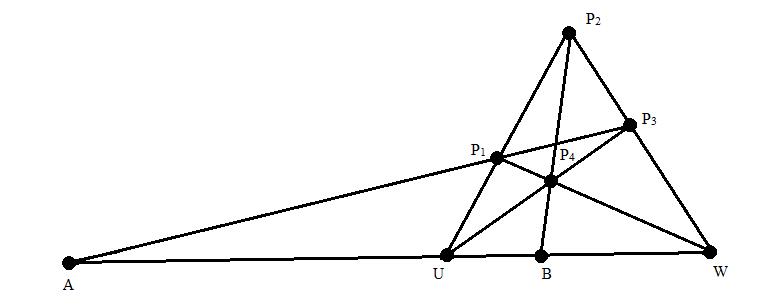
\includegraphics[width=1\textwidth]{authors/Stepanuk-1-fig-1.png}
        \caption{Четырёхвершинник с вершинами $P_1, P_2, P_3, P_4$}
        \label{fig:Stepanuk-1-fig-1}
    \end{minipage}
\hfill
    \begin{minipage}[h]{0.28\linewidth}
        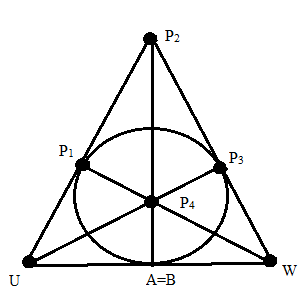
\includegraphics[width=1\textwidth]{authors/Stepanuk-1-fig-2.png}
        \caption{Четырёхвершинник Фано}
        \label{fig:Stepanuk-1-fig-2}
    \end{minipage}


  \end{center}
%\end{changemargin}

\end{figure}


\clearpage


Исследование полуполевой проективной плоскости  показало, что существуют такие множества пяти точек общего положения, для которых количество образованных этими точками четырёхвершинников Фано и обыкновенных четырёхвершинников принимают всевозможные значения. В~частности, используя точки $P_1 \bigl((1,0);(\upalpha,\upbeta);(1,\upalpha)\bigr)$, $P_2 \bigl((1,0);(\upbeta,\upbeta);(\upbeta,\upbeta)\bigr)$, $P_3 \bigl((1,0);(\upbeta,0);(\upbeta,0)\bigr)$, $P_4 \bigl((1,0);(0,0);(\upbeta,1)\bigr)$, $P_5 \bigl((1,0);(1,1);(0,\upbeta)\bigr)$,  получаем 5~четырёхвершинников, причём все они являются обыкновенными.

В общем случае пять точек общего положения образовывают пять  четырёхвершинников, из которых $k$ четырёхвершинников являются обыкновенные, а остальные $(5-k)$ являются четырёхвершинниками Фано. Выявлено, что $k$ может принимать все возможные значения от~0 до~5. Примеры таких точек общего положения представлены в табл.~3.

\begin{table}[H]
    \begin{changemargin}{-2.4cm}{0cm}
\caption{Примеры множества точек общего положения}
\end{changemargin}
\label{tab:my-table}
\begin{center}
\begin{tabular}{m{4.5cm}m{2.7cm}m{2.7cm}}
  \toprule
\parbox[c][][c]{0.3\textwidth}{ \centeringТочки} & \parbox[c][][c]{0.2\textwidth}{ \centeringОбык\-но\-вен\-ные четырёх\-вершинники} & \parbox[c][][c]{0.2\textwidth}{ \centeringЧетырёх\-вершинники Фано} \\
\midrule
$P_1 = \bigl((1,0);(0,\upalpha);(\upalpha,1)\bigr)$\newline
                $P_2 = \bigl((1,0);(\upbeta,\upbeta);(1,0)\bigr)$\newline
                $P_3 = \bigl((0,0);(0,0);(1,0)\bigr)$\newline
                $P_4 = \bigl((0,0);(1,0);(0,1)\bigr)$\newline
                $P_5 = \bigl((1,0);(\upbeta,1);(0,\upalpha)\bigr)$
      &
      &            $P_1P_2P_3P_4$ \newline
                      $P_1P_2P_3P_5$\newline
                        $P_1P_2P_5P_4$\newline
                        $P_1P_5P_3P_4$\newline
                        $P_5P_2P_3P_4$             \\
\midrule

$P_1 = \bigl((1,0);(\upalpha,\upalpha);(\upalpha,\upalpha)\bigr)$\newline
$P_2 = \bigl((1,0);(\upbeta,\upalpha);(\upbeta,0)\bigr)$\newline
$P_3 = \bigl((1,0);(\upalpha,0);(0,0)\bigr)$\newline
$P_4 = \bigl((1,0);(0,1);(1,\upbeta)\bigr)$\newline
$P_5 = \bigl((0,0);(0,0);(1,0)\bigr)$     &
            $P_1P_2P_3P_4$                   &
                              $P_1P_2P_3P_5$\newline
                              $P_1P_2P_5P_4$\newline
                              $P_1P_5P_3P_4$\newline
                              $P_5P_2P_3P_4$                 \\

\midrule
$P_1 = \bigl((1,0);(1,0);(\upalpha,1)\bigr)$\newline
$P_2 = \bigl((1,0);(0,1);(\upbeta,\upalpha)\bigr)$\newline
$P_3 = \bigl((1,0);(1,0);(\upbeta,1)\bigr)$\newline
$P_4 = \bigl((0,0);(1,1);(0,\upbeta)\bigr)$\newline
$P_5 = \bigl((1,0);(0,\upalpha);(\upbeta,\upalpha)\bigr)$      &
                              $P_1P_2P_3P_5$\newline
                              $P_1P_2P_5P_4$&
                                              $P_1P_2P_3P_4$ \newline
                                              $P_1P_5P_3P_4$\newline
                                              $P_5P_2P_3P_4$\\
\midrule

$P_1 = \bigl((1,0);(0,1);(0,0)\bigr)$\newline
$P_2 = \bigl((1,0);(\upbeta,\upbeta);(\upbeta,\upbeta)\bigr)$\newline
$P_3 = \bigl((1,0);(\upbeta,0);(\upbeta,0)\bigr)$\newline
$P_4 = \bigl((1,0);(0,0);(\upbeta,1)\bigr)$\newline
$P_5 = \bigl((1,0);(1,1);(0,\upbeta)\bigr)$      &
                                  $P_1P_2P_3P_5$\newline
                                  $P_1P_5P_3P_4$\newline
                                  $P_5P_2P_3P_4$&
                                                          $P_1P_2P_3P_4$\newline
                                                          $P_1P_2P_5P_4$\\

\midrule
$P_1 = \bigl((1,0);(\upbeta,1);(1,1)\bigr)$\newline
$P_2 = \bigl((1,0);(\upbeta,\upbeta);(\upbeta,\upbeta)\bigr)$\newline
$P_3 = \bigl((1,0);(\upbeta,0);(\upbeta,0)\bigr)$\newline
$P_4 = \bigl((1,0);(0,0);(\upbeta,1)\bigr)$\newline
$P_5 = \bigl((1,0);(1,1);(0,\upbeta)\bigr)$      &
                                  $P_1P_2P_3P_4$\newline
                                  $P_1P_2P_3P_5$\newline
                                  $P_1P_2P_5P_4$\newline
                                  $P_5P_2P_3P_4$&
                                                            $P_1P_5P_3P_4$\\ \bottomrule\\
\end{tabular}
\end{center}
\end{table}


\clearpage
\textbf{Выводы}

Показано, что для любого множества точек существуют конфигурации, в которых число обыкновенных четырёхвершинников и четырёхвершинников Фано равно и
соответственно. Для каждого из~шести перечисленных случаев указано искомое множество пяти точек общего положения.




\begin{thebibliography}{99}

\bibitem{}\BibAuthor{Кравцова~О.~В., Дураков~Б.~К.} Полуполевые плоскости нечётного порядка, допускающие подгруппу автотопизмов, изоморфную $A_5$ // Сиб. матем. журн.~--- 2018.~--- Т.~59, №~2.~--- С.~396--411.
\bibitem{}\BibAuthor{Шарафутдинова~А.~М.} Полный список полных $k$-дуг в проективной плоскости порядка 9 над правым почти-полем для $k=8, 9, 10$ // Вестн. Южно-Ур. ун-та. Сер. Математика Мех. Физ.~--- 2014.~--- Т.~6, №~2.~--- С.~77--79.
\bibitem{}\BibAuthor{Шатохин~Н.~Л.} Реперные изоморфизмы аффинных ельмслевовых плоскостей и $\upomega$ изотопии АН-тернаров // Владикавк. матем. журн.~--- 2007.~--- Т.~9, №~4.~--- С.~49--55.
\bibitem{}\BibAuthor{Штуккерт~П.~К.} Квазиполя и проективные плоскости трансляций малых чётных порядков~// Известия Иркутского государственного университета. Сер. Математика.~--- 2014.~--- №~7.~--- С.~141--159.
\bibitem{}\BibAuthor{Knuth~D.~E.} Finite semifields and projective planes~// J. Algebra.~--- 1965. ~--- Vol.~2.~--- P.~182--217.
\bibitem{}\BibAuthor{Menichetti~G.} $n$-dimensional algebras over a finite field with a cyclic extension of degree $n$ // Geom. Dedicata.~--- 1996.~--- Vol.~63.~--- P.~69--94.


\end{thebibliography}
